\usetikzlibrary{positioning,arrows.meta}

\begin{figure}[p]
\centering
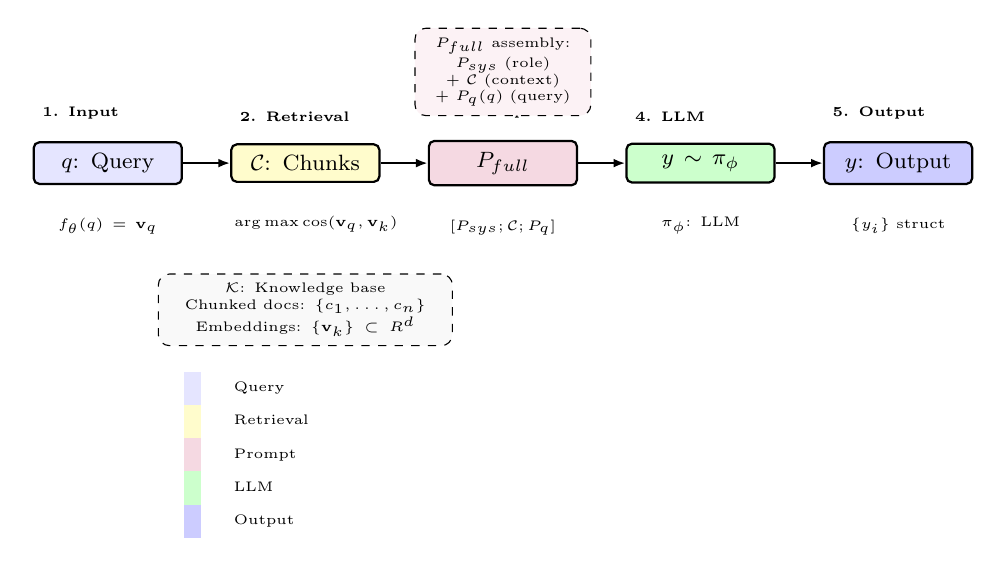
\begin{tikzpicture}[
  font=\footnotesize,
  block/.style={draw=black, rounded corners=2pt, thick, align=center, inner sep=4pt},
  arrow/.style={-{Latex[length=1.5mm]}, thick},
  formula/.style={font=\tiny, align=center, text width=1.8cm},
  node distance=0.8cm and 0.6cm
]

% ============================================================
% Main pipeline boxes (horizontal)
% ============================================================
\node[block, fill=blue!10, text width=1.6cm] (q) {$q$: Query};
\node[block, fill=yellow!20, text width=1.6cm, right=of q] (r) {$\mathcal{C}$: Chunks};
\node[block, fill=purple!15, text width=1.6cm, right=of r] (p) {$P_{\text{full}}$};
\node[block, fill=green!20, text width=1.6cm, right=of p] (l) {$y \sim \pi_\phi$};
\node[block, fill=blue!20, text width=1.6cm, right=of l] (o) {$y$: Output};

% Arrows
\draw[arrow] (q) -- (r);
\draw[arrow] (r) -- (p);
\draw[arrow] (p) -- (l);
\draw[arrow] (l) -- (o);

% ============================================================
% Stage labels above
% ============================================================
\node[font=\tiny\bfseries, above=0.15cm of q.north west, anchor=south west] {1. Input};
\node[font=\tiny\bfseries, above=0.15cm of r.north west, anchor=south west] {2. Retrieval};
\node[font=\tiny\bfseries, above=0.15cm of p.north west, anchor=south west] {3. Prompt};
\node[font=\tiny\bfseries, above=0.15cm of l.north west, anchor=south west] {4. LLM};
\node[font=\tiny\bfseries, above=0.15cm of o.north west, anchor=south west] {5. Output};

% ============================================================
% Formulas below each box
% ============================================================
\node[formula, below=0.3cm of q] (fq) {$f_\theta(q)=\mathbf{v}_q$};
\node[formula, below=0.3cm of r] (fr) {$\arg\max\cos(\mathbf{v}_q,\mathbf{v}_k)$};
\node[formula, below=0.3cm of p] (fp) {$[P_{\text{sys}};\mathcal{C};P_q]$};
\node[formula, below=0.3cm of l] (fl) {$\pi_\phi$: LLM};
\node[formula, below=0.3cm of o] (fo) {$\{y_i\}$ struct};

% ============================================================
% Knowledge base annotation (below retrieval formula)
% ============================================================
\node[draw=black, dashed, rounded corners, fill=gray!5, font=\tiny, below=0.4cm of fr, text width=3.5cm, align=center] (kb) {
$\mathcal{K}$: Knowledge base \\
Chunked docs: $\{c_1,\dots,c_n\}$ \\
Embeddings: $\{\mathbf{v}_k\}\subset\mathbb{R}^d$
};

% ============================================================
% Prompt composition detail (above prompt box)
% ============================================================
\node[draw=black, dashed, rounded corners, fill=purple!5, font=\tiny, above=0.3cm of p, text width=2cm, align=center] (pd) {
$P_{\text{full}}$ assembly: \\
$P_{\text{sys}}$ (role) \\
$+$ $\mathcal{C}$ (context) \\
$+$ $P_q(q)$ (query)
};

% ============================================================
% Legend (bottom left)
% ============================================================
\node[font=\tiny, anchor=north west, yshift=-0.2cm] at (kb.south west) {
\begin{tabular}{cl}
\colorbox{blue!10}{\strut} & Query \\
\colorbox{yellow!20}{\strut} & Retrieval \\
\colorbox{purple!15}{\strut} & Prompt \\
\colorbox{green!20}{\strut} & LLM \\
\colorbox{blue!20}{\strut} & Output
\end{tabular}};

\end{tikzpicture}

\caption{Pipeline architecture. The clinician query $q$ is embedded to $\mathbf{v}_q$, retrieves top-$k$ chunks $\mathcal{C}$ via cosine similarity from knowledge base $\mathcal{K}$, assembles full prompt $P_{\text{full}}$, and generates structured response $y$ via LLM $\pi_\phi$.}
\label{fig:model_architecture}
\end{figure}
